\clearpage
\appendix

\section{Per-scene training-view qualitative comparison}
\label{app:per_scene_train}

Figures~\ref{fig:supp_s0_f135}--\ref{fig:supp_s2_f300} show per-scene
side-by-side $|\mathrm{RA}|$ renders for all four methods on every
training frame, plus the held-out test frame ($F$, last column with the
red header). Rows are GT, mm3DGS (Ours), RadarSplat, Radar Fields, and
DART (cascaded). Per-cell test/train CC is overlaid in white.

These figures complement the aggregate train and test tables in the
main paper (Tables~\ref{tab:test_ra} and~\ref{tab:train_ra}) and confirm
visually that mm3DGS preserves wall and vehicle structure across all
eight training frames as well as the held-out test frame, while the
three baselines exhibit the characteristic failure modes discussed in
Sec.~\ref{sec:experiments:test}: RadarSplat over-smooths azimuth,
Radar Fields fails to reach the data with its hash-grid+MLP, and DART
is data-starved at the cascade radar's 16 chirps per frame.

\begin{figure}[h]
\centering
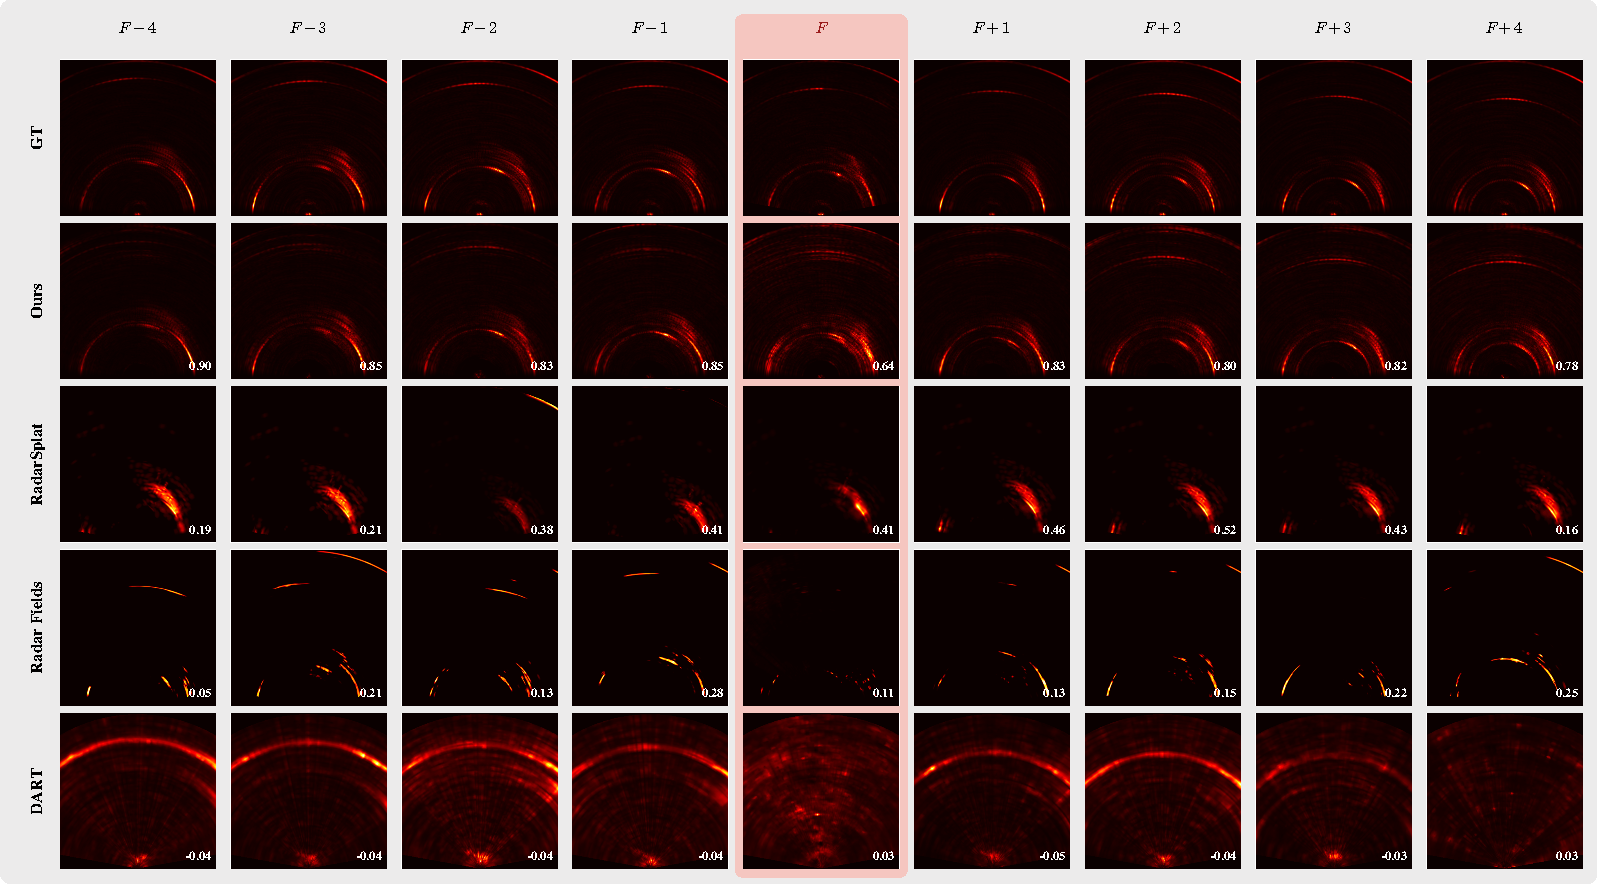
\includegraphics[width=\linewidth]{figs/supplement/supplement_seq_0_frame_135.pdf}
\caption{\textbf{Per-frame $|\mathrm{RA}|$ comparison, scene S0\,F135.}
Columns: 8 training frames ($F\!\pm\!1\!\ldots\!\pm\!4$, black headers)
and 1 held-out test frame ($F$, red header). Rows: GT, mm3DGS (Ours),
RadarSplat, Radar Fields, DART. Per-cell CC overlaid.}
\label{fig:supp_s0_f135}
\end{figure}

\begin{figure}[h]
\centering
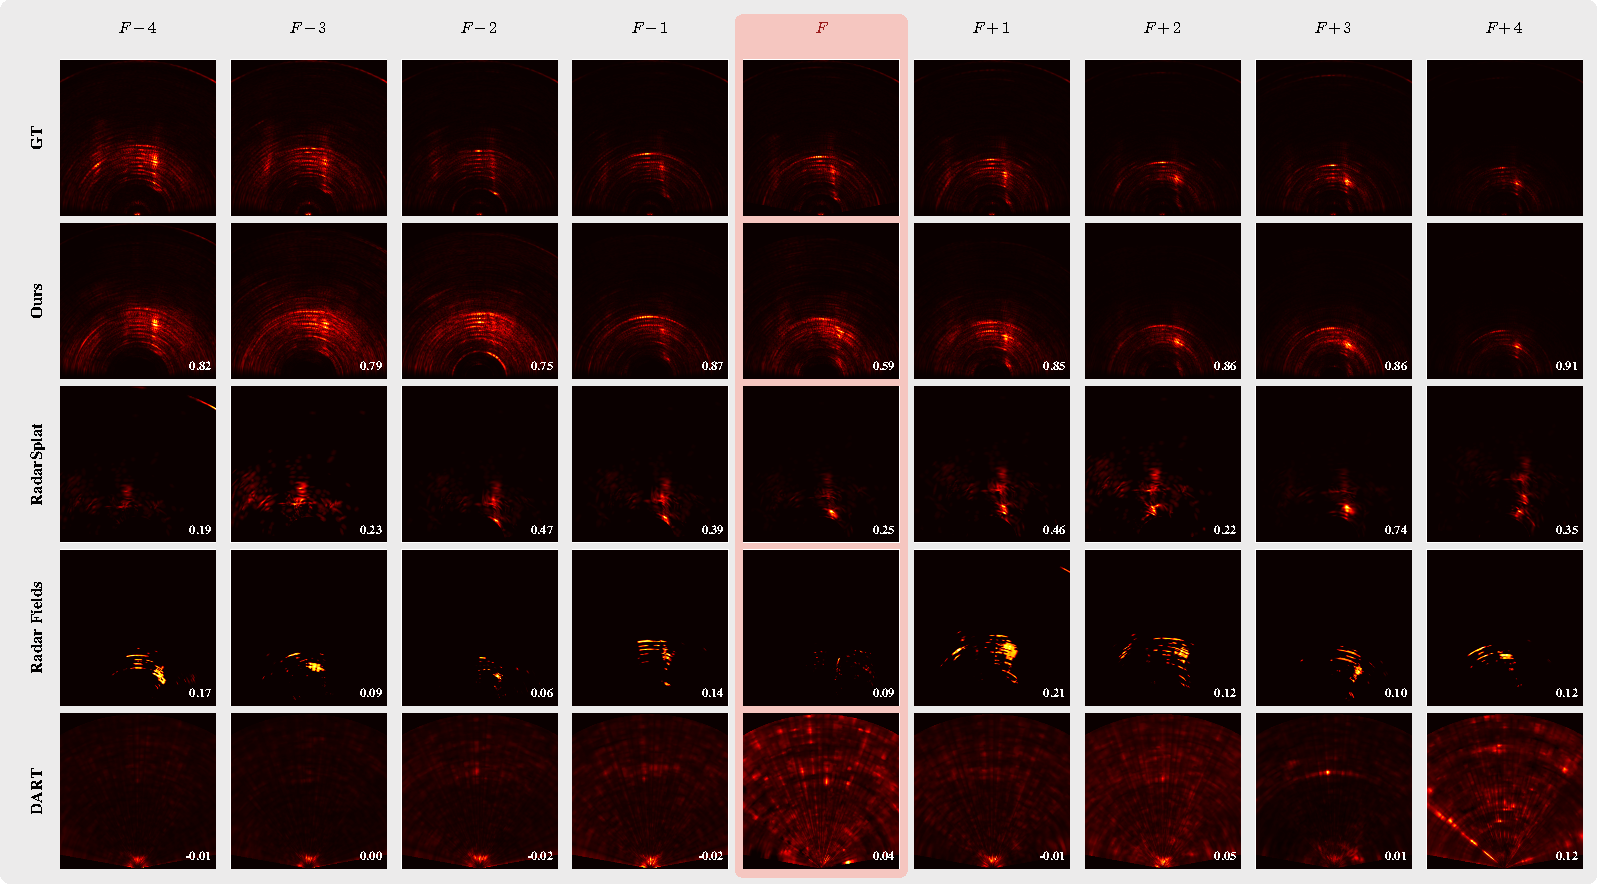
\includegraphics[width=\linewidth]{figs/supplement/supplement_seq_1_frame_185.pdf}
\caption{\textbf{Per-frame $|\mathrm{RA}|$ comparison, scene S1\,F185.}}
\label{fig:supp_s1_f185}
\end{figure}

\begin{figure}[h]
\centering
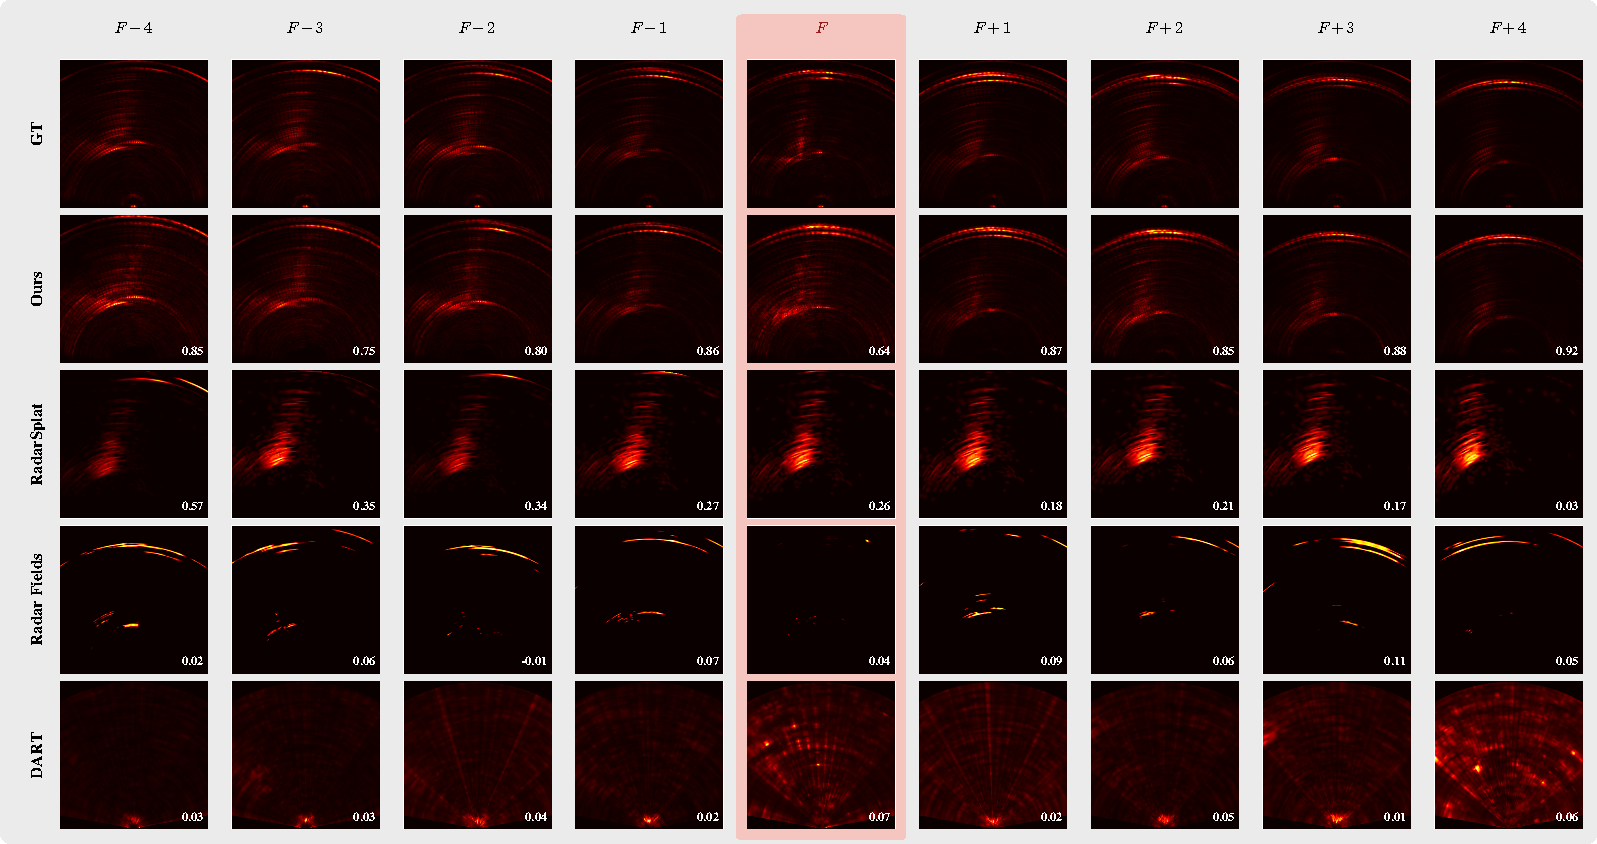
\includegraphics[width=\linewidth]{figs/supplement/supplement_seq_1_frame_438.pdf}
\caption{\textbf{Per-frame $|\mathrm{RA}|$ comparison, scene S1\,F438.}}
\label{fig:supp_s1_f438}
\end{figure}

\begin{figure}[h]
\centering
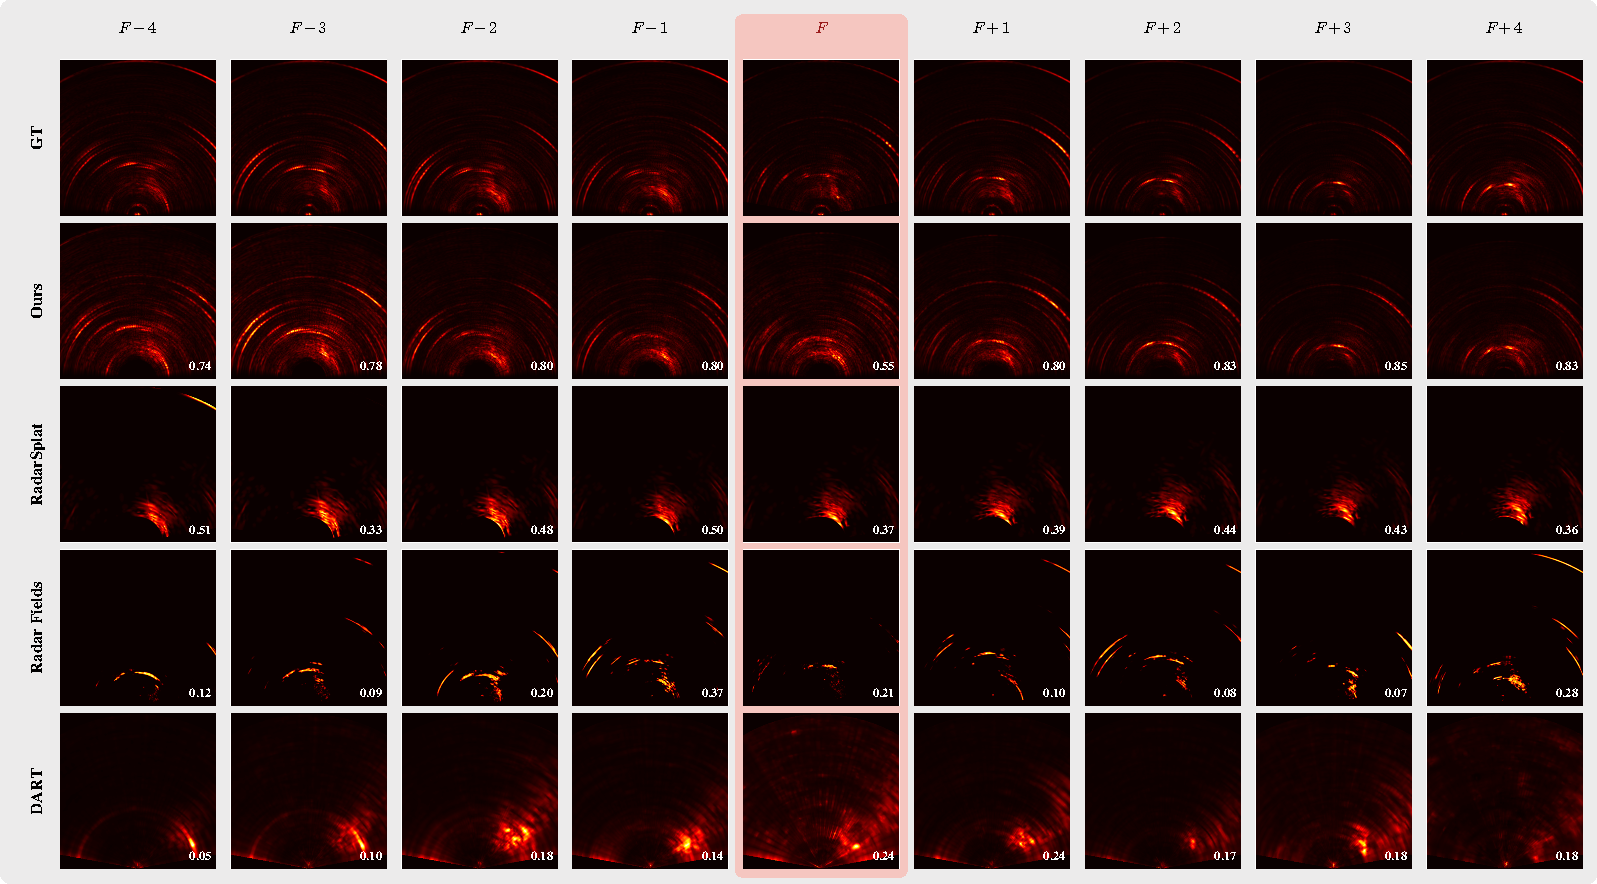
\includegraphics[width=\linewidth]{figs/supplement/supplement_seq_2_frame_105.pdf}
\caption{\textbf{Per-frame $|\mathrm{RA}|$ comparison, scene S2\,F105.}}
\label{fig:supp_s2_f105}
\end{figure}

\begin{figure}[h]
\centering
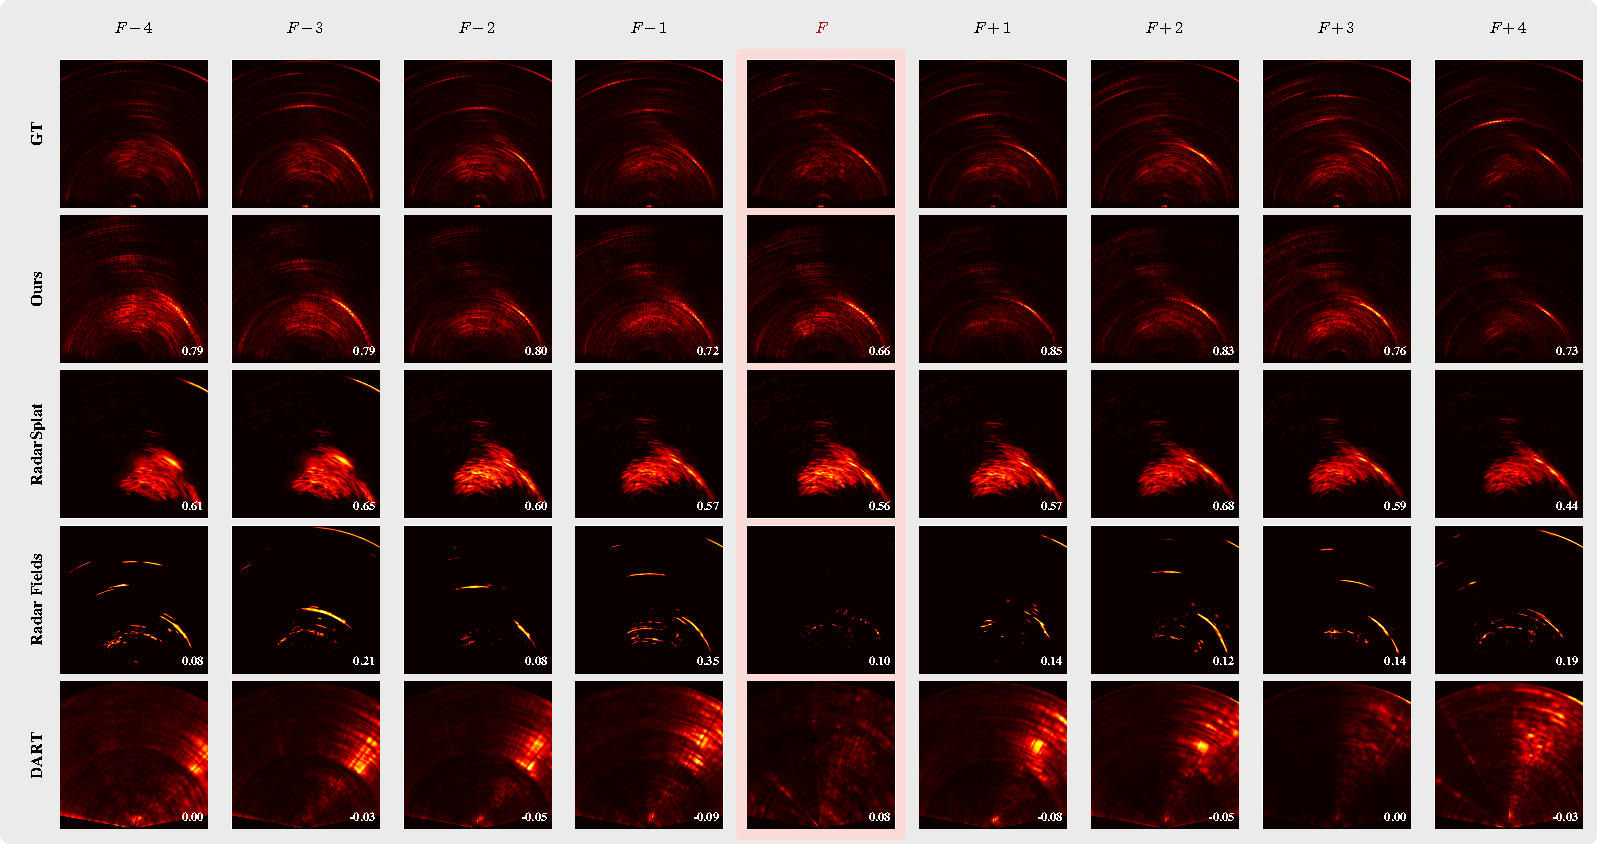
\includegraphics[width=\linewidth]{figs/supplement/supplement_seq_2_frame_160.pdf}
\caption{\textbf{Per-frame $|\mathrm{RA}|$ comparison, scene S2\,F160.}}
\label{fig:supp_s2_f160}
\end{figure}

\begin{figure}[h]
\centering
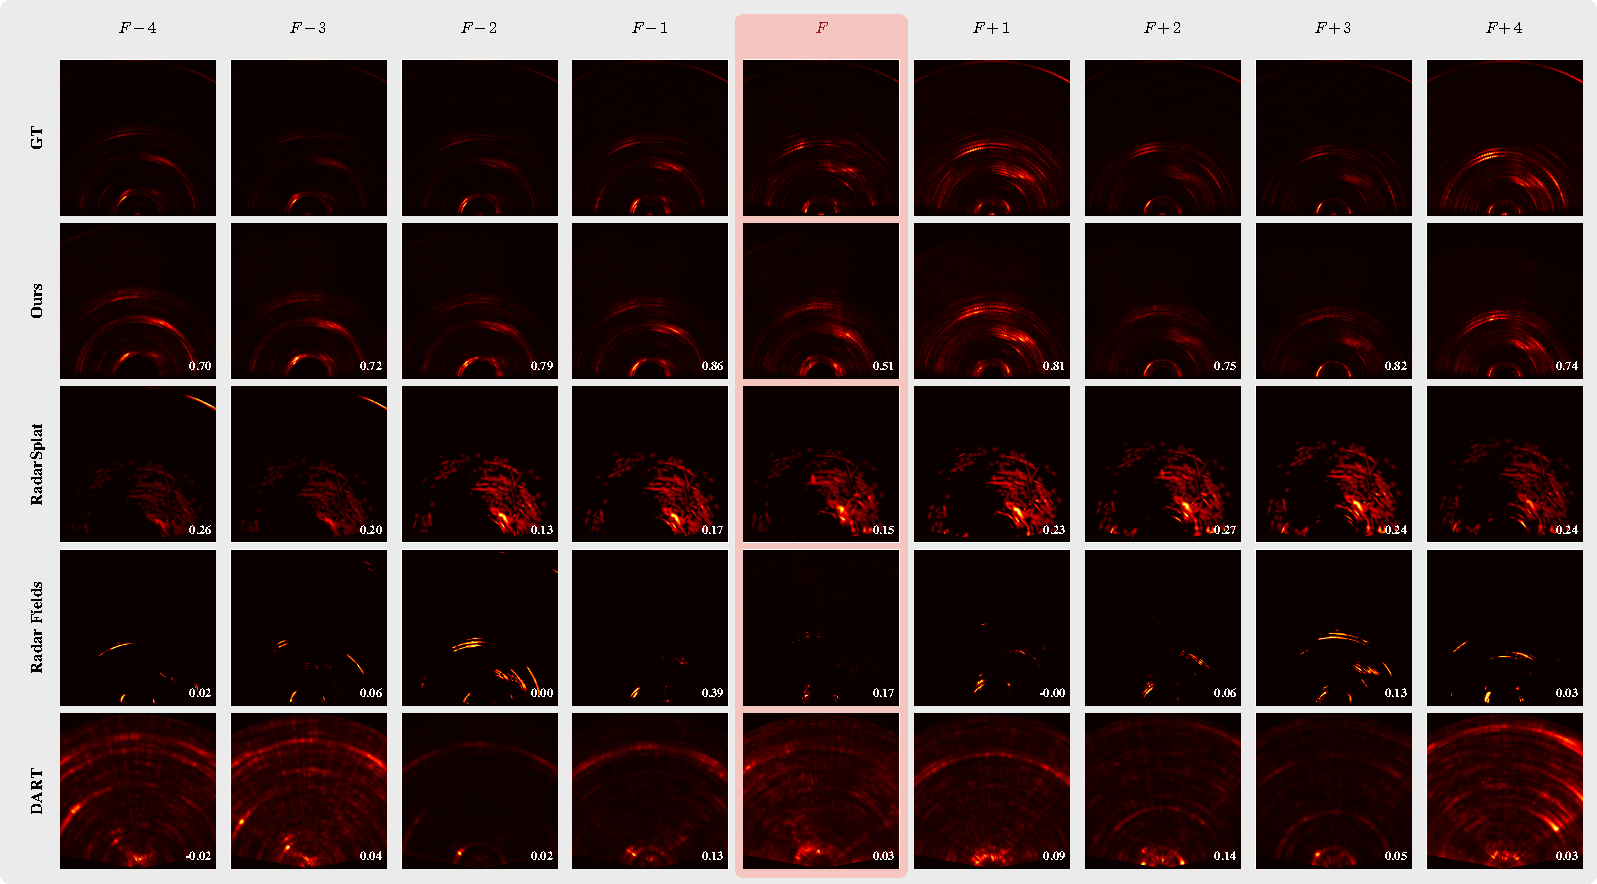
\includegraphics[width=\linewidth]{figs/supplement/supplement_seq_2_frame_300.pdf}
\caption{\textbf{Per-frame $|\mathrm{RA}|$ comparison, scene S2\,F300.}}
\label{fig:supp_s2_f300}
\end{figure}
